\documentclass{standalone}
\usepackage{graphicx}
\usepackage{tikz}
\usetikzlibrary{arrows,automata}
\begin{document}
    \scalebox{2.0}{
    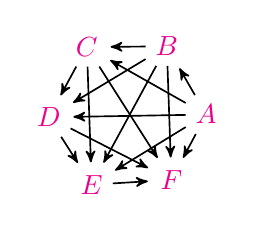
\begin{tikzpicture}[->,>=stealth',shorten >=1pt,auto,node distance=2.8cm, semithick]
      \tikzstyle{every state}=[fill=mymagenta,draw=none,text=white]
  
      \node[color=magenta] (v0) at (0:1) {$A$};
      \node[color=magenta] (v1) at (60:1) {$B$};
      \node[color=magenta] (v2) at (121:1) {$C$};
      \node[color=magenta] (v3) at (182:1) {$D$};
      \node[color=magenta] (v4) at (243:1) {$E$};
      \node[color=magenta] (v5) at (304:1) {$F$};
      \path (v0) edge (v1);
             \path (v0) edge (v2);
             \path (v0) edge (v3);
             \path (v0) edge (v4);
             \path (v0) edge (v5);
             \path (v1) edge (v2);
             \path (v1) edge (v3);
             \path (v1) edge (v4);
             \path (v1) edge (v5);
             \path (v2) edge (v3);
             \path (v2) edge (v4);
             \path (v2) edge (v5);
             \path (v3) edge (v4);
             \path (v3) edge (v5);
             \path (v4) edge (v5);
             \end{tikzpicture}
    }
\end{document}